\documentclass[border=20pt]{standalone}

\usepackage{tikz}
\usepackage{xcolor}

\definecolor{vblack}{HTML}{1a1a1a}
\definecolor{vgray}{HTML}{686868}
\definecolor{vblue}{HTML}{007acc}

\begin{document}
	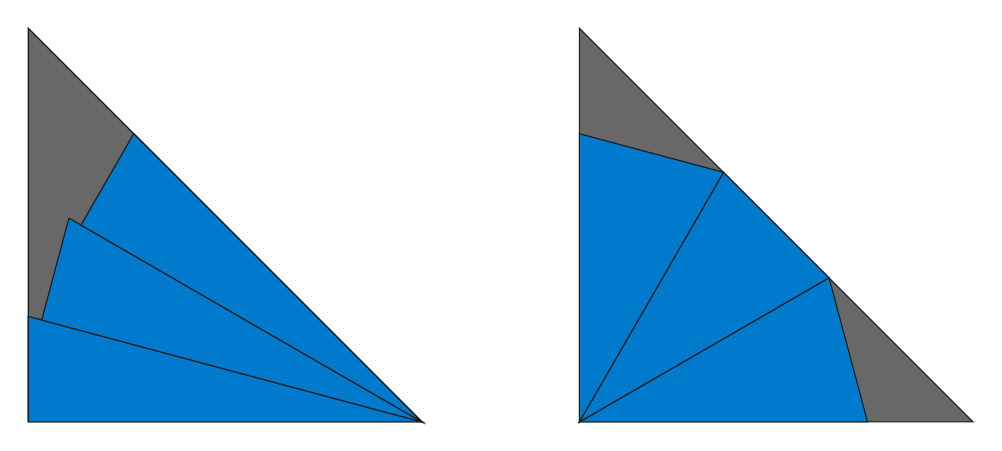
\begin{tikzpicture}
		\draw[draw = vblack, fill = vgray] (0,0) -- (0,5) -- (5,0) -- cycle;
		\draw[draw = vblack, fill = vblue] (5,0) -- (0,0) -- (0,1.3397) -- cycle;
		\draw[draw = vblack, fill = vblue] (5,0) -- (.17037, 1.2941) -- (.5171,2.5882) -- cycle;
		\draw[draw = vblack, fill = vblue] (5,0) -- (.6699,2.5) -- (1.3397,3.66) -- cycle;
		\draw [draw = vblack, fill = vgray] (7,0) -- (7,5) -- (12,0) -- cycle;
		\draw [draw = vblack, fill = vblue] (7,0) -- (10.66,0) -- (10.17,1.83) -- cycle;
		\draw [draw = vblack, fill = vblue] (7,0) -- (10.17,1.83) -- (8.83,3.17) -- cycle;
		\draw [draw = vblack, fill = vblue] (7,0) -- (8.83,3.17) -- (7,3.66) -- cycle;
	\end{tikzpicture}
\end{document}